\chapter{Исследовательский раздел}\label{sec:exp}
Раздел содержит технические характеристики устройства, на котором проведен эксперимент. Также раздел содержит результаты проведенного эксперимента.
\section{Технические характеристики}
Тестирование выполнялось на устройстве со следующими техническими характеристиками:
\begin{itemize}
	\item операционная система Ubuntu 20.04.1 LTS; \cite{linux}
	\item память 8 GiB;
	\item процессор AMD Ryzen 5 3500u.\cite{ryzen}
\end{itemize}

\section{Постановка эксперимента}
Эксперимент заключается в генерации гистограмм на основе клю­чей и соответствующих им количеств сравнений для поиска ключа.
Для каждого из алгоритмов строятся гистограммы 2 видов: для гистограммы первого типа отсортировать ключи по алфавиту, а для вто­рой - по количеству сравнений.
По полученным гистограммам необходимо сделать выводы об эф­фективности алгоритмов.Необходимо также отметить среднее, минимальное и максималь­ное количество сравнений.
Во время тестирования устройство было подключено к блоку питания и не нагружено никакими приложениями, кроме встроенных приложений окружения, окружением и системой тестирования. Оптимизация компилятора была отключена.

\section{Результаты эксперимента}
На рисунках 4.2 - 4.7 представлены результаты эксперимента.
По оси Х откладываются значения ключей, для оси У - количество сравнений.
Зеленой горизонтальной линеей отмечено минимальное количе­ство сравнений, желтой - среднее, красной - максимальное.

\begin{landscape}
	\begin{figure}[H]
		\centering
		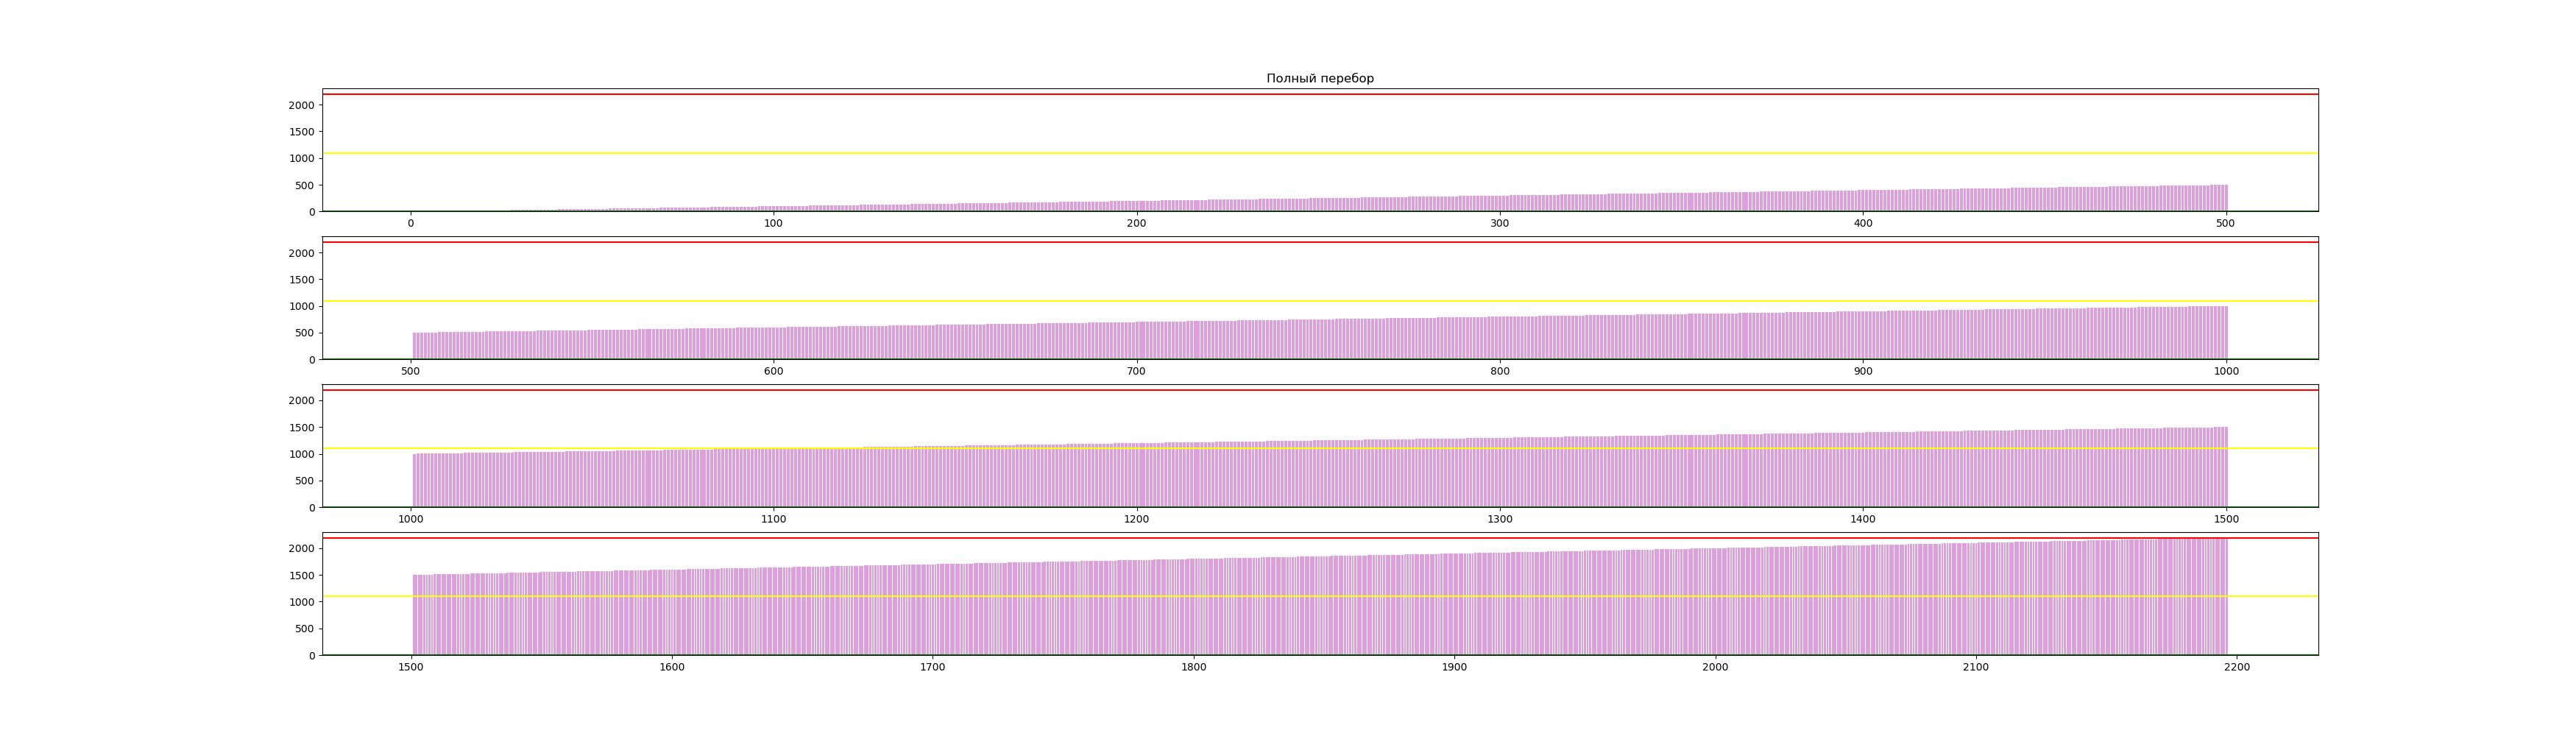
\includegraphics[width=0.95\linewidth]{assets/brute_force_keys.png}
		\caption{Полный перебор}
		\label{fig:brute_cmps}
		%\end{figure}
		%\begin{figure}[H]
		\centering
		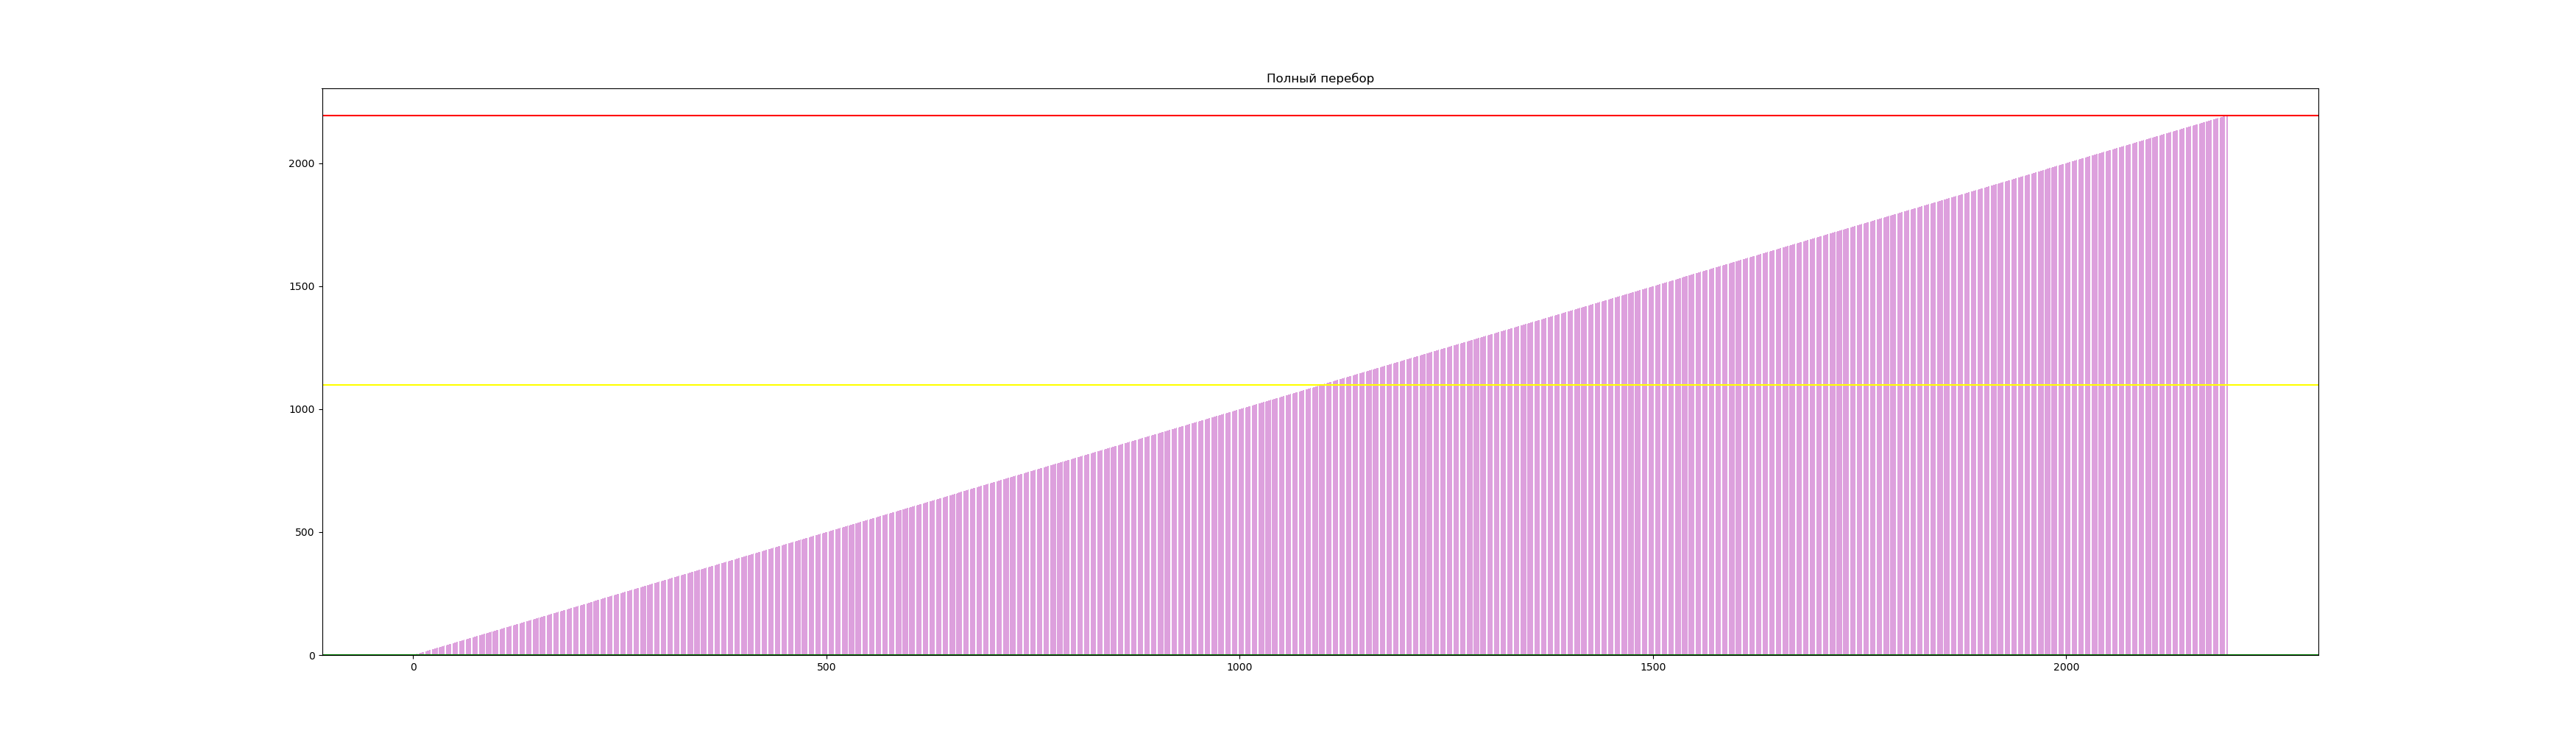
\includegraphics[width=0.95\linewidth]{assets/brute_force_cmps.png}
		\caption{Полный перебор}
		\label{fig:brute_keys}
	\end{figure}
\end{landscape}

\begin{landscape}
	\begin{figure}[H]
		\centering
		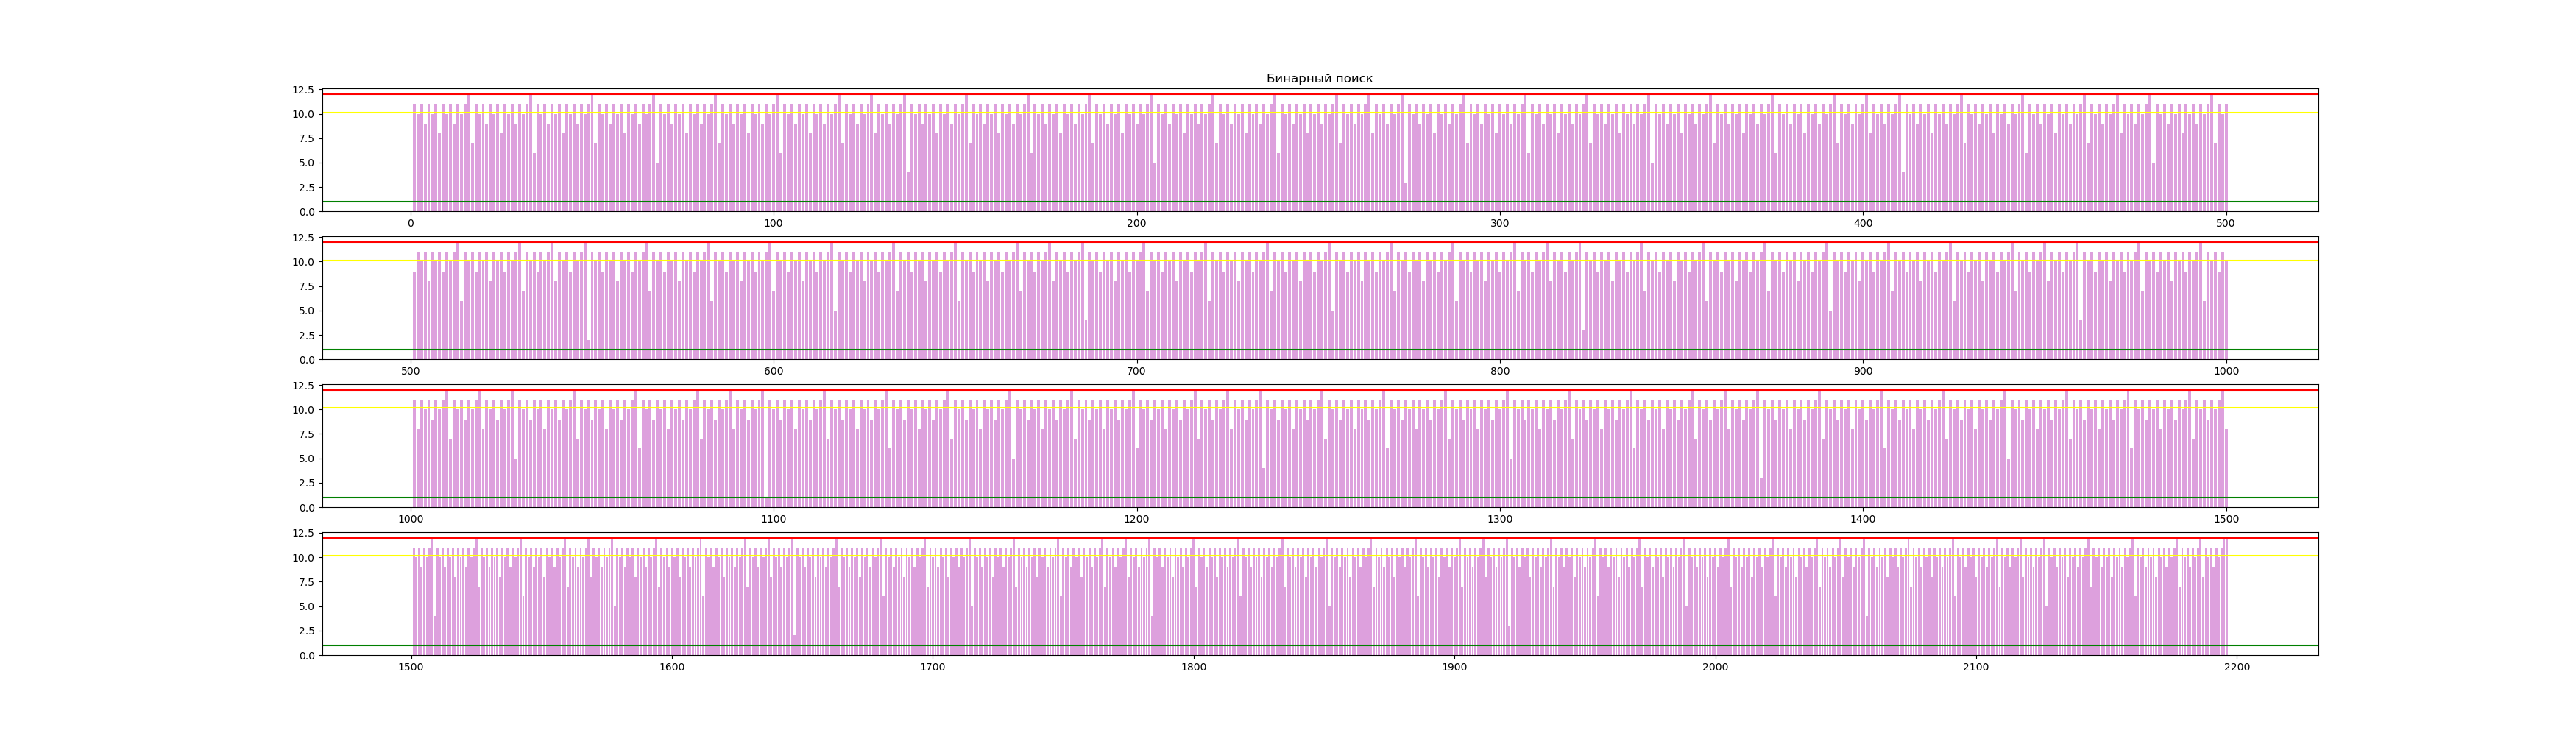
\includegraphics[width=0.95\linewidth]{assets/binary_search_keys.png}
		\caption{Бинарный поиск}
		\label{fig:binary_cmps}
		
		\centering
		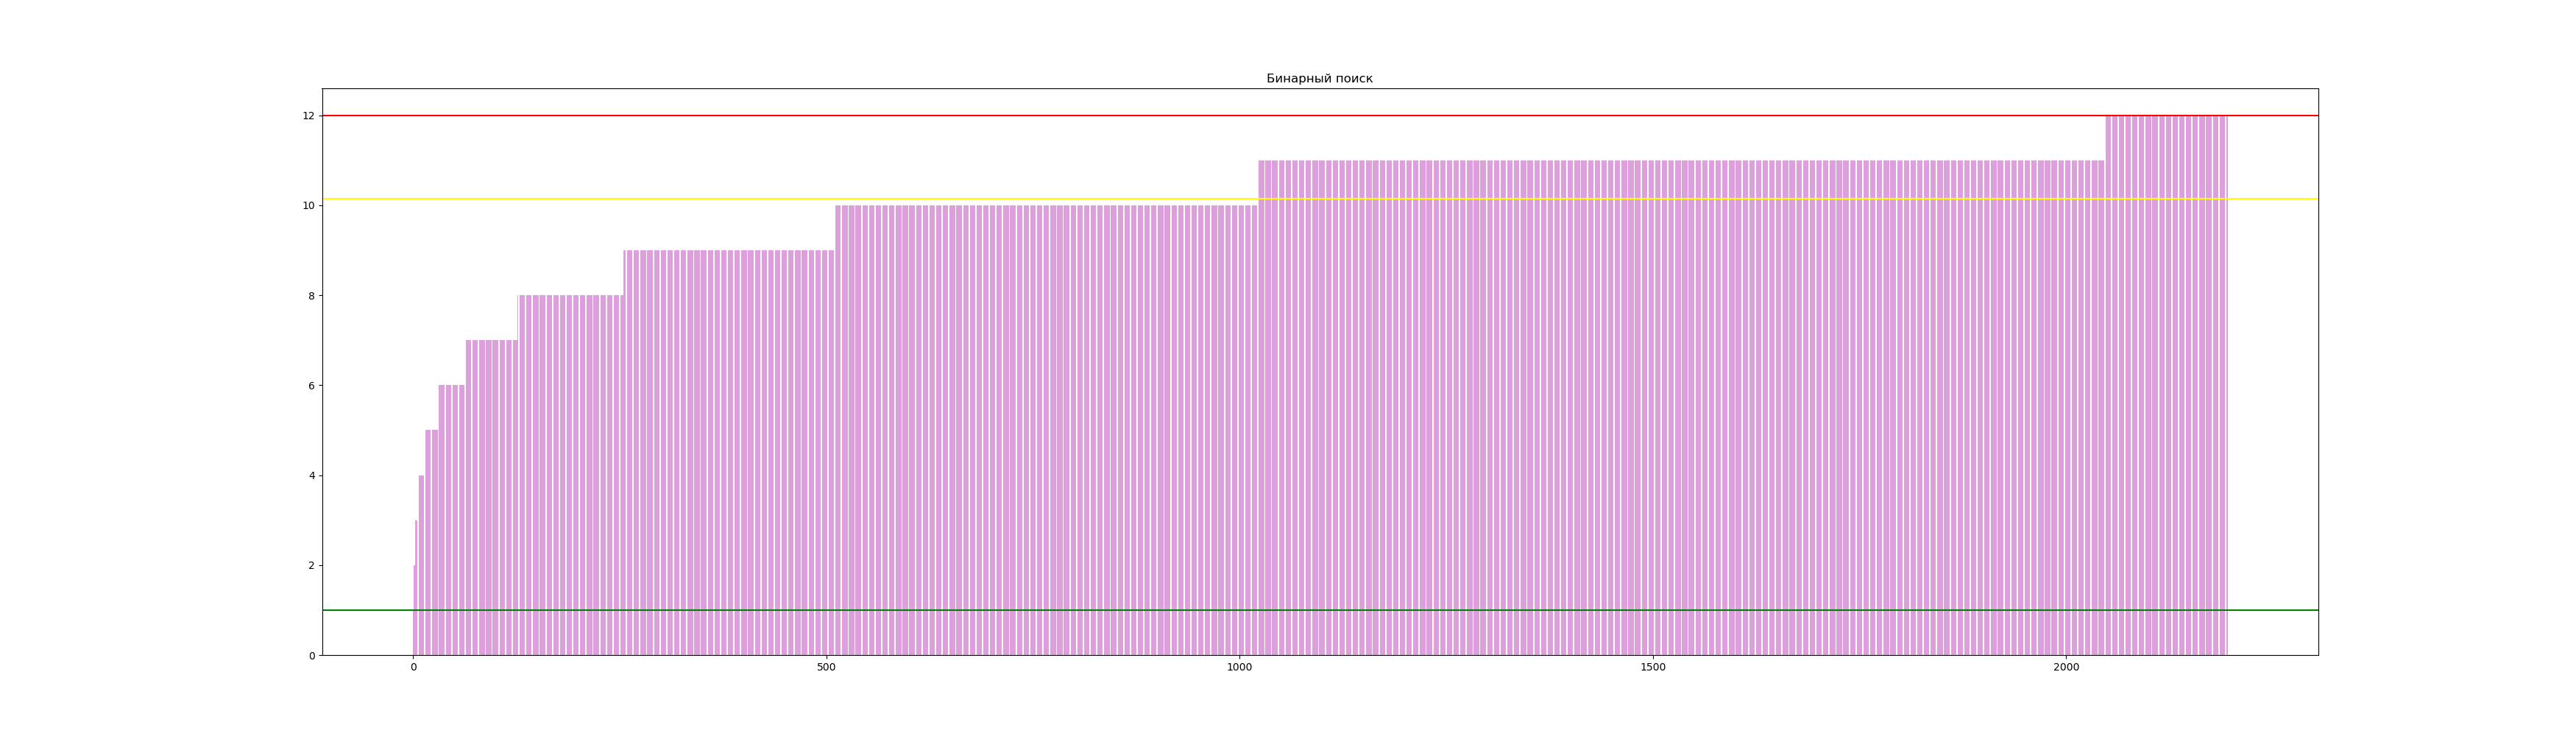
\includegraphics[width=0.95\linewidth]{assets/binary_search_cmps.png}
		\caption{Бинарный поиск}
		\label{fig:binary_keys}
	\end{figure}
\end{landscape}

\begin{landscape}
	\begin{figure}[H]
		\centering
		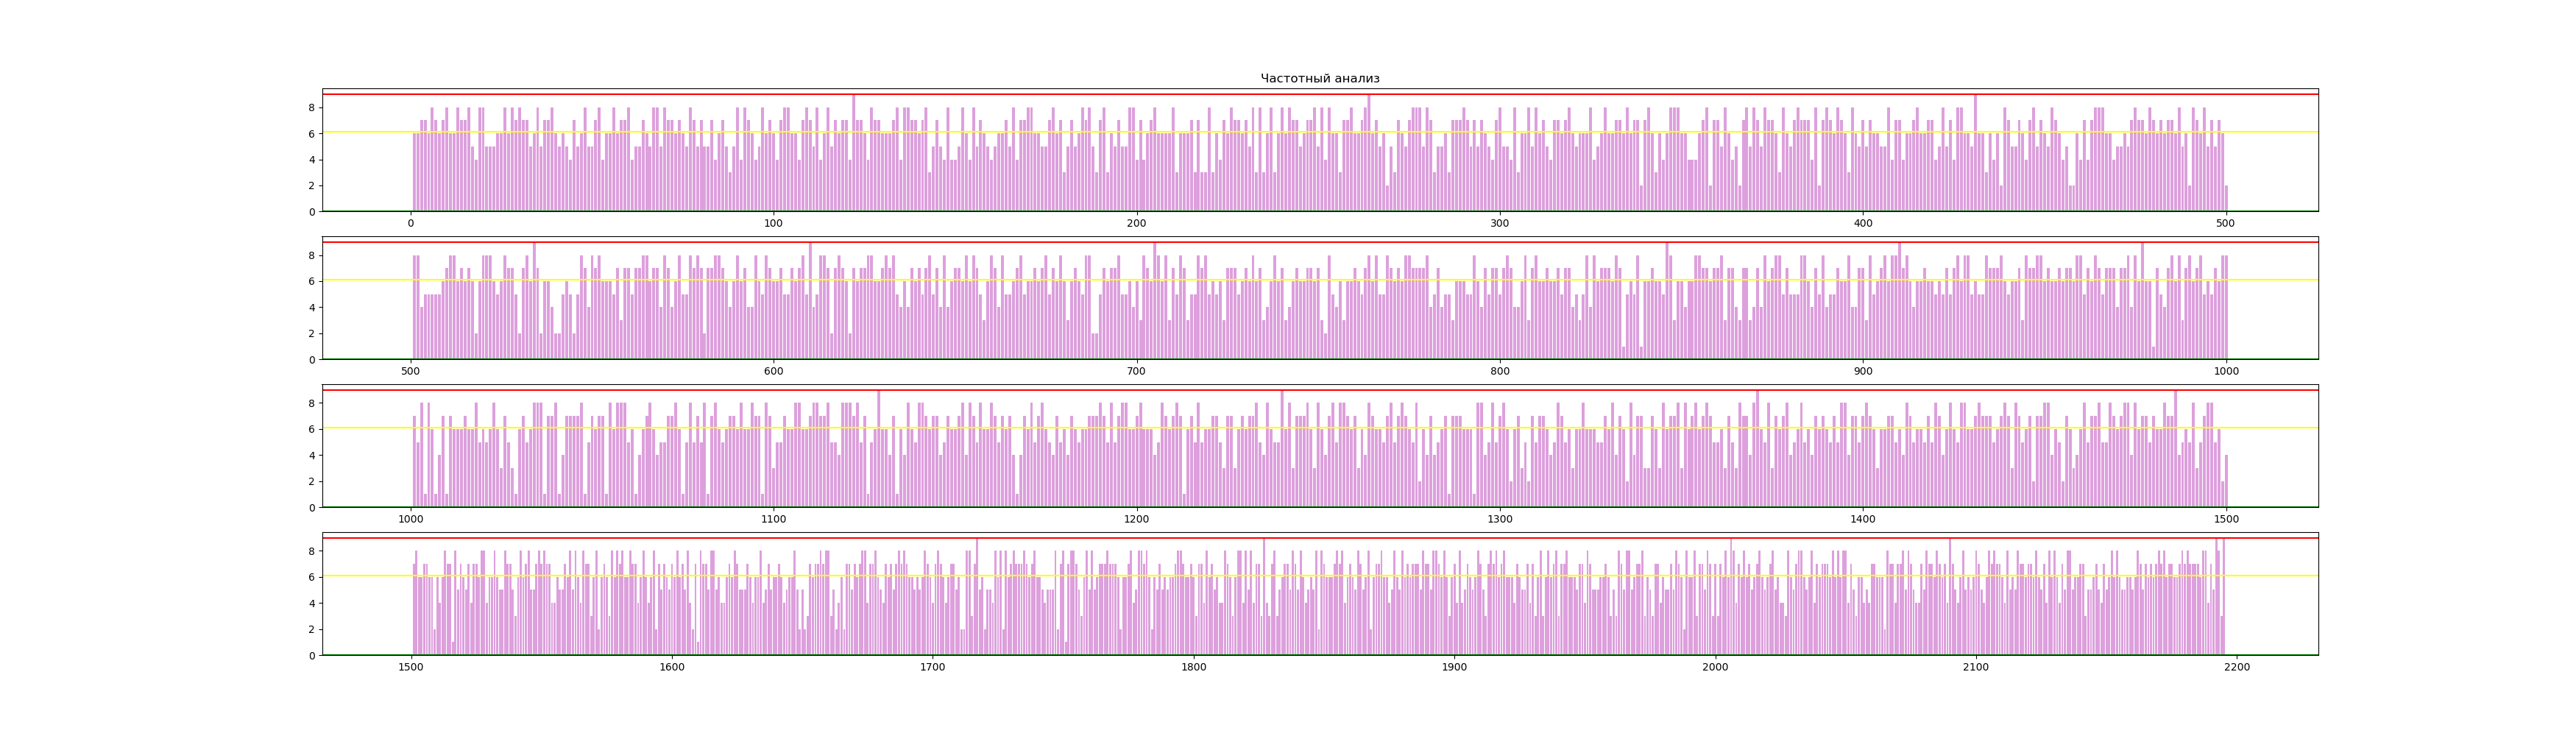
\includegraphics[width=0.95\linewidth]{assets/frequency_keys.png}
		\caption{Бинарный поиск}
		\label{fig:frequency_cmps}
		
		\centering
		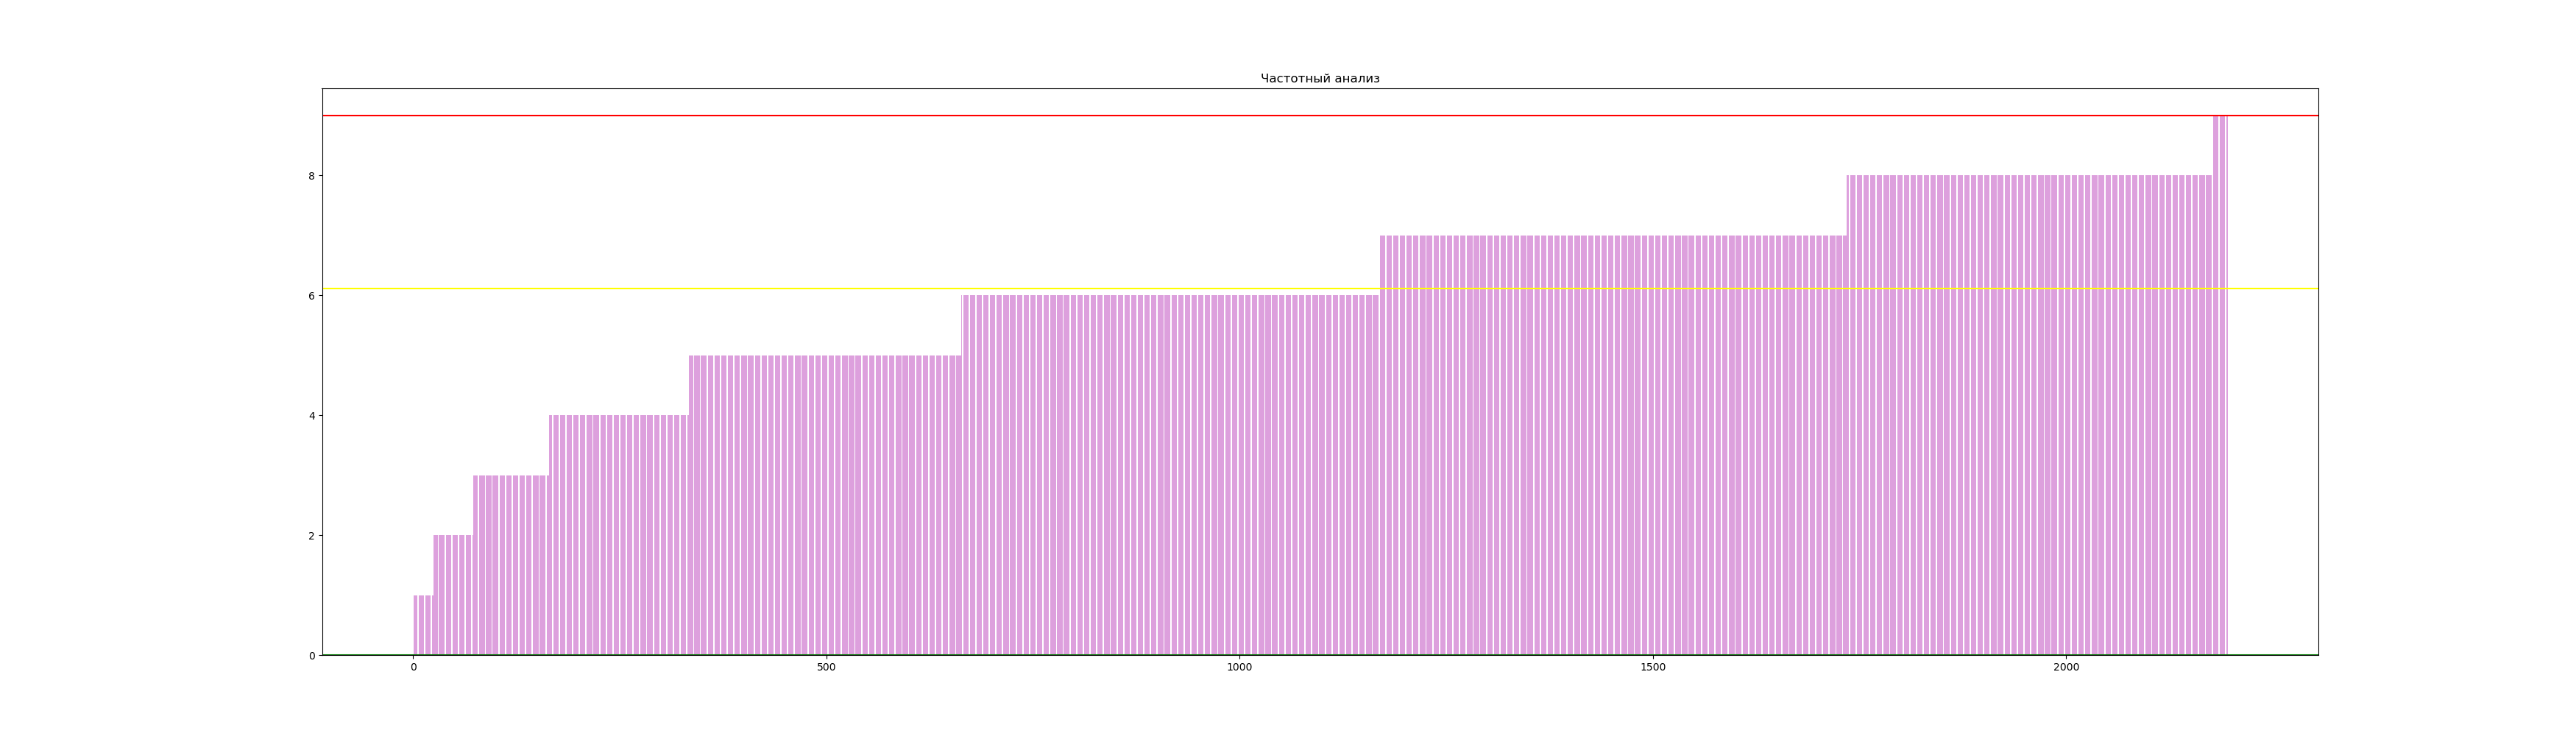
\includegraphics[width=0.95\linewidth]{assets/frequency_cmps.png}
		\caption{Бинарный поиск}
		\label{fig:frequency_keys}
	\end{figure}
\end{landscape}

\section{Вывод}\label{sec:exp-sum}
Как видно из графиков, частотный анализ требует в среднем тре­бует в 1.5-2 раза меньше сравнений. Как и ожидалось, алгоритм полного перебора требует наибольшего количества сравнений из всех представ­ленных алгоритмов.
Также видно, что гистограмма типа 1 для полного перебора - воз­растающая последовательность, в то время как для алгоритма бинарно­го поиска и, в частности, алгоритма частотного анализа, последователь­ность не является монотонно возрастающей в виду идеи работы алгорит­ма бинарного поиска.